
%% Original Software Publication article for Elsevier's `elsarticle' class
%% Target journal: Neurocomputing

\documentclass[preprint,12pt,a4paper]{elsarticle}

% -------------------------
% Packages
% -------------------------
\usepackage[a4paper,margin=2.5cm]{geometry}
\usepackage{amssymb}
\usepackage{amsmath}
\usepackage{graphicx}
\graphicspath{{figures/}}
\usepackage{subcaption}
\usepackage{placeins}
\usepackage[font=small,labelfont=bf]{caption}
\usepackage{tabularray}
\usepackage{booktabs,tabularx,makecell,threeparttable,adjustbox}
\usepackage{array}
\usepackage[table]{xcolor}
\definecolor{rowgray}{gray}{0.96}
\newcommand{\best}[1]{\textbf{#1}}
\newcommand{\second}[1]{\underline{#1}}
\usepackage{xurl}
\usepackage[hidelinks]{hyperref}
\usepackage{tikz}
\usetikzlibrary{arrows.meta,positioning,backgrounds}


% Replace these before submission after creating the GitHub repository and Zenodo archive.
\newcommand{\theratimeRepository}{\url{https://github.com/USERNAME/theratime}}
\newcommand{\theratimeZenodo}{DOI to be inserted after Zenodo archival}

\journal{Neurocomputing}

\begin{document}

\begin{frontmatter}

\title{TheraTime: a reliability-aware software framework for therapeutic timing evaluation in mental-health response retrieval}
\author[label1]{Asmae Briouya\corref{cor1}}
\cortext[cor1]{Corresponding author.}
\ead{asmae.briouya@uit.ac.ma}
\author[label1]{Hasnae Briouya}


\author[label1]{Ali Choukri}
\author[label1]{Mohamed Amnai}

\affiliation[label1]{organization={Laboratory of Computer Sciences},
             addressline={Faculty of Sciences},
             city={Kenitra},
             country={Morocco}}

\begin{abstract}
Mental-health response retrieval is usually evaluated using semantic relevance or retrieval rank, but these measures do not directly assess whether a retrieved response is therapeutically appropriate for the user's current need. A response may be semantically related to a user query while still being poorly timed, for example by giving advice before validation, missing a safety concern, or offering only empathy when the user explicitly asks for concrete steps. This paper presents TheraTime, an offline software framework for therapeutic timing evaluation in mental-health response retrieval.

TheraTime separates response evaluation into three transparent components: support-stage classification for the user query, support-move classification for the retrieved response, and rule-based timing assessment through a stage--move compatibility taxonomy. The framework uses pre-trained sentence-transformer encoders and prototype descriptions rather than supervised fine-tuning. Dense retrieval uses all-MiniLM-L6-v2, while the default timing classifiers use paraphrase-mpnet-base-v2, reducing circular encoder bias between retrieval and timing evaluation. The software evaluates TF-IDF, BM25, and dense retrieval baselines over ESConv, CounselChat, and MentalChat16K, and reports top-1 timing accuracy (TTA@1), timing precision over the top \(k\), Hit@\(k\), timing error categories, confidence margins, stress-test behavior, inter-annotator agreement, post-hoc calibration, and selective reliability analysis.

In an illustrative experiment with 2250 query-level retrieval examples and 11250 ranked judgments, BM25 achieved the strongest top-1 timing performance (TTA@1 = 0.6053), followed by TF-IDF (0.5760) and dense MiniLM retrieval (0.4187). The default MPNet timing system achieved TTA@1 = 0.5333 across all retrieval methods, outperforming a MiniLM timing ablation (0.3898) and a keyword-stage ablation (0.4564). A five-case stress test behaved as designed, with TTA@1 = 0.20, TTP@2 = 0.60, and Hit@2 = 1.00. Human validation on 150 shared examples showed substantial agreement for support-stage correctness (\(\kappa=0.7999\)) and support-move correctness (\(\kappa=0.6930\)), and moderate agreement for timing-label correctness (\(\kappa=0.5234\)). Conservative post-hoc calibration improved TTA@1 from 0.5333 to 0.5573, and selective reliability filtering further increased accepted-subset TTA@1 to 0.5872 at 80\% coverage, flagging 448 of 2250 rank-1 cases for human review.

TheraTime is not a clinical decision-support system and is not validated for deployment with real users. It is released as a research-oriented offline evaluation framework for studying when retrieved mental-health responses are appropriately timed, where uncertain or safety-sensitive cases can be routed to human review.
\end{abstract}

\begin{keyword}
Mental-health response retrieval \sep Therapeutic timing \sep Emotional support dialogue \sep Reliability calibration \sep Selective prediction \sep Human annotation
\end{keyword}

\end{frontmatter}

% =========================================================
% ====================== MANUSCRIPT =======================
% =========================================================

\section{Motivation and significance}
\label{sec:intro}

Conversational systems are increasingly studied for emotional support and mental-health assistance. Datasets such as ESConv, CounselChat, and MentalChat16K provide examples of help-seeker queries and supportive responses, making it possible to study retrieval and response generation in this domain~\cite{Liu2021ESConv,Bertagnolli2018CounselChat,Xu2025MentalChat16K}. This direction has become more urgent with the rapid growth of large language models (LLMs) in mental-health applications. Recent reviews highlight both potential benefits and major limitations, including inconsistent evaluation protocols, limited clinical validation, reliability concerns, ethical risks, and the need for standardized safety-focused benchmarks~\cite{Guo2024LLMMentalHealth,Hua2025ScopingLLMMentalHealth,Voultsiou2026LLMMentalHealth}. Existing retrieval evaluation often focuses on semantic similarity, rank, or overlap with a reference answer. These measures are useful, but they do not fully capture the timing of support.

In mental-health support, the same response type can be appropriate in one context and poorly timed in another. Practical advice can be helpful when a user explicitly asks for steps, but it may be premature when the user is overwhelmed and first needs validation or grounding. Empathy can be appropriate for distress disclosure, but insufficient when the user is asking for specific actions. Safety referral is essential when the user expresses self-harm risk. These distinctions suggest that response retrieval should be evaluated not only by semantic relatedness, but also by whether the retrieved response delivers the right support move at the right moment.

Recent empirical work reinforces this need for specialized evaluation. Studies of LLM responses in mental-health settings have examined empathy, motivational-interviewing adherence, demographic disparities, and crisis response, showing that surface-level fluency does not guarantee safe or equitable support~\cite{Gabriel2024CanAIRelate,Sorin2024LLMEmpathy}. Safety studies have also reported that chatbot agents may fail to respond adequately to simulated suicidal-risk scenarios or may rate potentially inappropriate suicide-related responses more favorably than experts~\cite{Pichowicz2025ChatbotSuicide,Heston2025SIRI}. These findings motivate evaluation methods that are narrower than general helpfulness and that explicitly inspect safety-sensitive response properties.

This paper introduces TheraTime, an offline software framework for therapeutic timing evaluation in mental-health response retrieval. The framework is designed around four goals:

\begin{itemize}
    \item \textbf{Timing-aware evaluation.} TheraTime evaluates whether a retrieved response is compatible with the user's support stage, rather than only whether it is semantically similar.
    \item \textbf{Transparent taxonomy.} User queries are mapped to support stages and retrieved responses to support moves. A rule engine assigns final timing labels from a stage--move compatibility table.
    \item \textbf{Model-agnostic retrieval comparison.} The framework evaluates TF-IDF, BM25, and dense retrieval under a shared timing evaluator.
    \item \textbf{Reliability-aware reporting.} Human annotation, conservative post-hoc calibration, and selective reliability analysis are included to avoid overclaiming automatic timing judgments.
\end{itemize}

TheraTime is explicitly designed as a research framework. It is not a therapy chatbot, does not provide clinical advice, and should not be deployed as a clinical decision-support tool. Its intended use is offline evaluation, error analysis, and reliability-aware benchmarking of retrieved mental-health responses.

\section{Software description}
\label{sec:software_description}

\subsection{Design goals}

TheraTime was developed to provide a reproducible and inspectable evaluation pipeline. Its design follows five principles:

\begin{itemize}
    \item \textbf{Separation of retrieval and timing evaluation.} Retrieval methods produce candidate responses, while the timing module evaluates their appropriateness.
    \item \textbf{Prototype-based classification.} Stage and move labels are inferred using pre-trained sentence-transformer encoders and natural-language prototype descriptions. No supervised fine-tuning is performed.
    \item \textbf{Transparent rule engine.} The final timing label is produced by an explicit compatibility table rather than by an opaque end-to-end classifier.
    \item \textbf{Stress testing and diagnostics.} The framework includes positive and negative control vignettes to verify whether obvious timing failures are detected.
    \item \textbf{Human-in-the-loop validation.} Annotation tools and kappa analysis scripts are provided to quantify inter-annotator agreement and support post-hoc calibration.
\end{itemize}

\subsection{Core architecture}

Figure~\ref{fig:framework_overview} summarises the TheraTime pipeline. The software begins by loading mental-health question-answer datasets, extracting valid query-response pairs, and building retrieval examples. Three retrieval backends are supported: TF-IDF, BM25, and dense retrieval with all-MiniLM-L6-v2. Retrieved responses are then evaluated by the timing module.

\begin{figure}[t]
\centering
\resizebox{0.92\linewidth}{!}{%
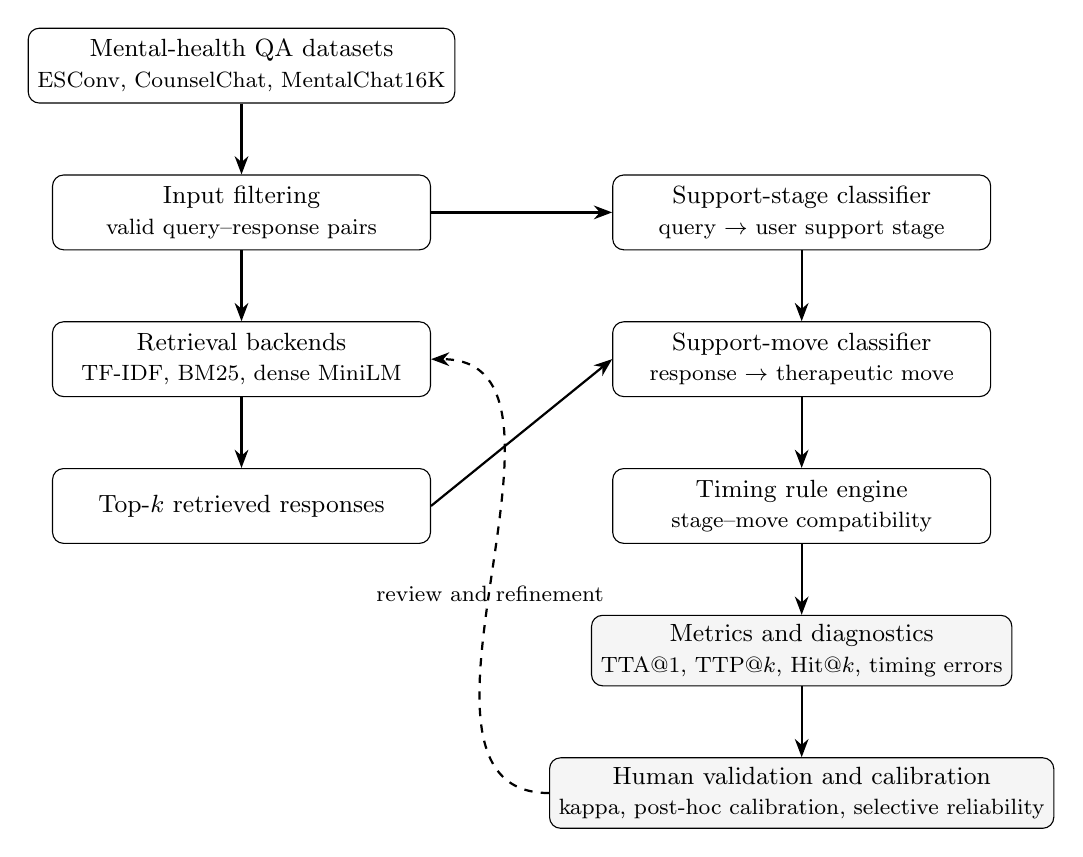
\begin{tikzpicture}[
    node distance=0.9cm,
    box/.style={
        rectangle,
        rounded corners=4pt,
        draw=black,
        align=center,
        minimum width=4.8cm,
        minimum height=0.95cm,
        fill=white,
        font=\small
    },
    smallbox/.style={
        rectangle,
        rounded corners=4pt,
        draw=black,
        align=center,
        minimum width=4.8cm,
        minimum height=0.85cm,
        fill=rowgray,
        font=\small
    },
    arrow/.style={-Stealth, thick},
    dashedarrow/.style={-Stealth, thick, dashed}
]

% Left column: retrieval pipeline
\node[box] (data) {Mental-health QA datasets\\
\footnotesize ESConv, CounselChat, MentalChat16K};

\node[box, below=of data] (filter) {Input filtering\\
\footnotesize valid query--response pairs};

\node[box, below=of filter] (retrieval) {Retrieval backends\\
\footnotesize TF-IDF, BM25, dense MiniLM};

\node[box, below=of retrieval] (candidates) {Top-\(k\) retrieved responses};

% Right column: timing evaluation
\node[box, right=2.3cm of filter] (stage) {Support-stage classifier\\
\footnotesize query \(\rightarrow\) user support stage};

\node[box, below=of stage] (move) {Support-move classifier\\
\footnotesize response \(\rightarrow\) therapeutic move};

\node[box, below=of move] (timing) {Timing rule engine\\
\footnotesize stage--move compatibility};

\node[smallbox, below=of timing] (metrics) {Metrics and diagnostics\\
\footnotesize TTA@1, TTP@\(k\), Hit@\(k\), timing errors};

\node[smallbox, below=of metrics] (calibration) {Human validation and calibration\\
\footnotesize kappa, post-hoc calibration, selective reliability};

% Arrows
\draw[arrow] (data) -- (filter);
\draw[arrow] (filter) -- (retrieval);
\draw[arrow] (retrieval) -- (candidates);

\draw[arrow] (filter.east) -- (stage.west);
\draw[arrow] (candidates.east) -- (move.west);

\draw[arrow] (stage) -- (move);
\draw[arrow] (move) -- (timing);
\draw[arrow] (timing) -- (metrics);
\draw[arrow] (metrics) -- (calibration);

\draw[dashedarrow] (calibration.west) to[out=180,in=0] node[below, font=\footnotesize] {review and refinement} (retrieval.east);

\end{tikzpicture}%
}
\caption{Overview of the TheraTime software framework. The left column shows data preparation and retrieval, while the right column shows therapeutic timing evaluation, diagnostics, human validation, and reliability-aware calibration.}
\label{fig:framework_overview}
\end{figure}

\subsection{Input filtering and datasets}
\label{subsec:datasets}

TheraTime operates on query-response pairs. Each input pair is filtered to remove greetings, fragments, very short responses, unusually long queries, and obvious non-informative artifacts. This reduces noise before retrieval and timing evaluation.

The illustrative experiment uses three public mental-health or emotional-support resources:

\begin{itemize}
    \item \textbf{ESConv.} A dataset of emotional support conversations designed around support strategies and help-seeker/supporter interactions~\cite{Liu2021ESConv}.
    \item \textbf{CounselChat.} A question-answer dataset derived from public counseling questions and therapist responses~\cite{Bertagnolli2018CounselChat}.
    \item \textbf{MentalChat16K.} A mental-health conversational assistance benchmark combining real anonymized interview data and synthetic dialogue data~\cite{Xu2025MentalChat16K}.
\end{itemize}

For each dataset, 800 valid pairs were extracted. The retrieval stage used up to 250 queries per dataset and per retrieval method, yielding 750 examples for each retrieval backend and 2250 query-level examples in total.

\subsection{Support-stage and support-move taxonomies}

TheraTime defines seven user support stages and nine response support moves. The stages are intended to represent the user's current need, while the moves represent what the response is doing.

\begin{table}[!htbp]
\centering
\small
\caption{TheraTime support-stage taxonomy.}
\label{tab:stages}
\rowcolors{2}{rowgray}{white}
\setlength{\tabcolsep}{5pt}
\renewcommand{\arraystretch}{1.15}
\begin{tabularx}{\linewidth}{p{3.8cm}X}
\toprule
\textbf{Stage} & \textbf{Meaning} \\
\midrule
distress\_disclosure & The user shares sadness, fear, loneliness, pain, or distress without yet asking for concrete help. \\
high\_emotional\_intensity & The user is overwhelmed, panicking, crying, spiraling, or emotionally dysregulated. \\
unclear\_need & The user is vague, confused, or unable to explain what is wrong. \\
advice\_seeking & The user explicitly asks for steps, strategies, coping techniques, or concrete actions. \\
psychoeducation\_seeking & The user asks why something is happening or requests an explanation. \\
crisis\_safety & The user states suicidal thoughts, self-harm intent, inability to stay safe, or urgent safety risk. \\
followup\_problem\_solving & The user has already received support and is now asking for planning or next steps. \\
\bottomrule
\end{tabularx}
\end{table}

\begin{table}[!htbp]
\centering
\small
\caption{TheraTime support-move taxonomy.}
\label{tab:moves}
\rowcolors{2}{rowgray}{white}
\setlength{\tabcolsep}{5pt}
\renewcommand{\arraystretch}{1.15}
\begin{tabularx}{\linewidth}{p{3.8cm}X}
\toprule
\textbf{Move} & \textbf{Meaning} \\
\midrule
validation & Acknowledges the user's feelings as understandable or valid. \\
empathy & Expresses warmth, care, and emotional presence. \\
reflective\_listening & Restates or mirrors the user's situation or feelings. \\
clarification & Asks a gentle question to better understand the user's need. \\
grounding & Helps the user calm down, breathe, stabilize, or focus on the present. \\
practical\_advice & Provides concrete coping steps, behavioral strategies, or action plans. \\
psychoeducation & Explains symptoms, emotional processes, or why feelings occur. \\
encouragement & Offers hope, reassurance, motivation, or affirmation. \\
safety\_referral & Directs the user toward emergency help, crisis support, a trusted person, or urgent safety resources. \\
\bottomrule
\end{tabularx}
\end{table}

\subsection{Prototype classifiers}

The timing module uses two prototype classifiers. The stage classifier maps the user query to one of the support stages. The move classifier maps the retrieved response to one of the support moves. Each label is represented by a short natural-language description. A sentence-transformer encoder embeds the input and the prototypes, and cosine similarity determines the predicted label.

The default timing encoder is \texttt{sentence-transformers/paraphrase-mpnet-base-v2}. Dense retrieval uses \texttt{sentence-transformers/all-MiniLM-L6-v2}. This separation is intentional: the retrieval model and the timing evaluator do not rely on the same default encoder, reducing circular bias between response selection and response assessment. Sentence-transformers are widely used to encode sentences into dense vectors for similarity and semantic search tasks~\cite{Reimers2019SentenceBERT}.

\subsection{Timing rule engine}
\label{subsec:timing_rule_engine}

Given a predicted stage \(s\) and a predicted move \(m\), TheraTime assigns a timing label using a rule-based compatibility table. The possible timing labels are:

\begin{itemize}
    \item \textbf{well\_timed}: the support move is compatible with the user's current support stage.
    \item \textbf{premature\_advice}: practical advice is given before validation, grounding, or clarification.
    \item \textbf{delayed\_safety}: safety risk is present but the response does not prioritize safety.
    \item \textbf{over\_validation}: the user asks for practical help but the response only validates, empathizes, or reflects.
    \item \textbf{missing\_clarification}: the user need is unclear but the response does not clarify.
    \item \textbf{stage\_mismatch}: the response move is incompatible with the predicted stage.
\end{itemize}

The core logic is transparent. For example, if \(s=\texttt{crisis\_safety}\) and \(m\notin\{\texttt{safety\_referral},\texttt{grounding},\texttt{validation}\}\), the timing label is \texttt{delayed\_safety}. If \(s=\texttt{unclear\_need}\) and the response gives practical advice instead of clarification or supportive presence, the label is \texttt{premature\_advice} or \texttt{missing\_clarification}, depending on the predicted move.

\subsection{Metrics and outputs}
\label{subsec:metrics}

TheraTime reports the following main metrics:

\begin{itemize}
    \item \textbf{TTA@1}: top-1 therapeutic timing accuracy, defined as the proportion of rank-1 retrieved responses labelled \texttt{well\_timed}.
    \item \textbf{TTP@\(k\)}: timing precision over the top \(k\) retrieved responses, defined as the mean well-timed rate across rank \(\leq k\).
    \item \textbf{Hit@\(k\)}: the proportion of queries for which at least one response in the top \(k\) is well-timed.
    \item \textbf{Timing error rates}: rates of \texttt{premature\_advice}, \texttt{delayed\_safety}, \texttt{over\_validation}, \texttt{missing\_clarification}, and \texttt{stage\_mismatch}.
    \item \textbf{Confidence diagnostics}: stage and move prototype margins, low-confidence flags, and entropy over prototype scores.
\end{itemize}

The framework exports CSV and JSON outputs, including all automatic judgments, method-level comparison tables, ablation tables, stress-test results, diagnostic reports, annotation files, inter-annotator agreement reports, post-calibration outputs, selective reliability tables, and publication-ready figures.

\section{Human validation, calibration, and selective reliability}
\label{sec:human_calibration}

\subsection{Human annotation protocol}

A standalone HTML annotation tool was used to validate a 150-example sample of rank-1 TheraTime judgments. The sample was proportionally stratified by automatic timing label, rather than sampled equally from each class. The final sample contained 53 \texttt{well\_timed}, 45 \texttt{stage\_mismatch}, 22 \texttt{premature\_advice}, 12 \texttt{over\_validation}, 10 \texttt{delayed\_safety}, and 8 \texttt{missing\_clarification} examples. Each annotator answered three questions:

\begin{enumerate}
    \item Is the predicted support stage correct for the user query?
    \item Is the predicted support move correct for the retrieved response?
    \item Is the automatic final timing label correct for the query-response pair?
\end{enumerate}

For each question, annotators selected \texttt{yes}, \texttt{no}, or \texttt{unsure}. If they selected \texttt{no} or \texttt{unsure}, they could provide a correction label and optional notes. Two annotators, Hasnae and Asmae, annotated the same 150 examples.

\subsection{Inter-annotator agreement}

Cohen's kappa was computed for the three binary correctness judgments after excluding no cases, because neither annotator used missing or unsure labels in the final files. Table~\ref{tab:kappa} reports the results. Following the common Landis and Koch interpretation, \(\kappa\) values between 0.61 and 0.80 are described as substantial, and values between 0.41 and 0.60 as moderate~\cite{Landis1977Kappa}.

\begin{table}[!htbp]
\centering
\caption{Inter-annotator agreement on 150 shared TheraTime annotation examples.}
\label{tab:kappa}
\small
\setlength{\tabcolsep}{5pt}
\renewcommand{\arraystretch}{1.15}
\rowcolors{2}{rowgray}{white}
\begin{tabularx}{\linewidth}{lcccc}
\toprule
\textbf{Question} &
\textbf{Observed} &
\textbf{Expected} &
\textbf{Cohen's \(\kappa\)} &
\textbf{Interpretation} \\
\midrule
Stage correctness  & 0.9000 & 0.5002 & 0.7999 & Substantial \\
Move correctness   & 0.8467 & 0.5005 & 0.6930 & Substantial \\
Timing correctness & 0.7867 & 0.5524 & 0.5234 & Moderate \\
\bottomrule
\end{tabularx}
\end{table}

The agreement results show that the stage and move categories are generally interpretable and reproducible. Timing correctness is more difficult, which is expected because it depends on both stage and move interpretation and on their interaction. The human validation results therefore support using TheraTime as a structured evaluation framework, while also motivating reliability-aware reporting.

\subsection{Human-validated automatic label accuracy}

Human validation also showed that automatic labels should not be treated as ground truth. Both annotators agreed that the automatic stage label was correct in 66 of 150 cases (44.0\%), the automatic move label in 67 of 150 cases (44.7\%), and the automatic timing label in 34 of 150 cases (22.7\%). These results indicate that the prototype and rule system is useful for producing first-pass diagnostic signals, but is not reliable enough to serve as a final automatic timing classifier. The lower timing accuracy relative to stage and move accuracy individually reflects error propagation: a correct stage or move judgment does not guarantee a correct timing label, because timing depends on the interaction between both components.

A correction-direction analysis further characterized the behavior of the automatic timing component. Among the 13 cases in which both annotators rejected the automatic timing label and both provided explicit timing corrections, 12 cases (92.3\%) were corrected to \texttt{well\_timed}, while only one case (7.7\%) remained genuinely mistimed under a different error subtype. This indicates that the automatic timing rule engine has a conservative over-flagging bias: it tends to mark candidate responses as mistimed even when human annotators judge them contextually acceptable. Consequently, TheraTime should be interpreted as a screening and diagnostic tool for surfacing candidate timing concerns, not as a final automatic timing classifier.


\begin{table}[!htbp]
\centering
\caption{Correction-direction analysis for cases where both annotators rejected the automatic timing label and both provided explicit timing corrections.}
\label{tab:correction_direction}
\rowcolors{2}{rowgray}{white}
\begin{tabular}{lrr}
\toprule
\textbf{Human correction direction} & \textbf{Count} & \textbf{Proportion} \\
\midrule
Corrected to \texttt{well\_timed} & 12 & 92.3\% \\
Still mistimed with different subtype & 1 & 7.7\% \\
\midrule
Total valid cases & 13 & 100.0\% \\
\bottomrule
\end{tabular}
\end{table}

\subsection{Post-hoc calibration}

TheraTime includes a post-hoc calibration module that uses human annotations as a lightweight correction layer. This module does not fine-tune the sentence-transformer encoders. Instead, it learns transparent correction rules from human consensus. Several strategies were evaluated:

\begin{itemize}
    \item \textbf{Human-rules direct}: directly maps automatic stage, move, and timing labels to common human corrections. This is treated as an overfit-risk ablation.
    \item \textbf{Human-rules recompute}: corrects stage and move labels, then recomputes timing using the rule engine.
    \item \textbf{Conservative human recompute}: requires stronger support and same-correction agreement before applying stage or move rules.
    \item \textbf{Hybrid isotonic-conservative}: combines conservative stage/move correction, timing recomputation, and isotonic reliability estimates.
\end{itemize}

Table~\ref{tab:calibration} summarises the calibration results. The direct rule method achieved an apparent TTA@1 of 1.0000 and is therefore excluded from the main claim due to overfit risk. The conservative and hybrid methods are more defensible because they avoid directly forcing timing labels and instead recompute timing from calibrated stage--move pairs. The correction-direction results in Table~\ref{tab:correction_direction} further show why calibration should be treated as a reliability layer: many automatic timing rejections are corrected by humans to \texttt{well\_timed}, so the system is better used for screening and prioritising review than for final automatic classification.

The conservative recompute and hybrid isotonic-conservative methods produced identical TTA@1 because they applied the same conservative stage--move correction rules; the hybrid variant additionally stores isotonic reliability estimates for the selective reliability analysis. The conservative and hybrid methods changed 204 rank-1 stage labels, 986 rank-1 move labels, and 1070 rank-1 timing labels. The direct rule method changed 1050 rank-1 timing labels and is therefore reported only as an overfit-risk ablation.

\begin{table}[!htbp]
\centering
\caption{Main post-hoc calibration comparison. The direct rule method is retained as an ablation only because it directly changes timing labels and shows overfit risk.}
\label{tab:calibration}
\small
\setlength{\tabcolsep}{5pt}
\renewcommand{\arraystretch}{1.18}
\rowcolors{2}{rowgray}{white}
\begin{tabularx}{\linewidth}{lcccX}
\toprule
\textbf{Method} & \textbf{TTA@1} & \textbf{Gain} & \textbf{Risk} & \textbf{Use in paper} \\
\midrule
Baseline & 0.5333 & 0.0000 & Low--moderate & Main baseline \\
Confidence only & 0.5333 & 0.0000 & Low--moderate & Uncertainty flag only \\
Human rules direct & 1.0000 & 0.4667 & High & Ablation only \\
Human rules recompute & 0.5556 & 0.0222 & Low--moderate & Diagnostic \\
Conservative recompute & \best{0.5573} & \best{0.0240} & Low--moderate & Main calibrated result \\
Hybrid isotonic-conservative & \best{0.5573} & \best{0.0240} & Low--moderate & Recommended reliability-aware variant \\
\bottomrule
\end{tabularx}
\end{table}

\subsection{Selective reliability analysis}
\label{subsec:selective_reliability}

Because mental-health timing judgments are subjective and potentially safety-sensitive, TheraTime includes selective reliability analysis. Instead of forcing every automatic judgment to be accepted, the system ranks judgments by a reliability score and flags low-reliability cases for human review. This is aligned with selective prediction, where a model may abstain on uncertain inputs to improve the risk--coverage trade-off~\cite{Geifman2019SelectiveNet}. Calibration and confidence estimation are also motivated by the broader neural calibration literature, where post-hoc methods are used to better align confidence with correctness likelihood~\cite{Guo2017Calibration}. Conformal prediction offers a related model-agnostic approach to uncertainty quantification, although the current TheraTime implementation uses simpler risk--coverage analysis rather than formal conformal guarantees~\cite{Campos2024ConformalNLP}.

The selected reliability score was the minimum of the stage and move confidence margins. This is conservative because final timing depends on both components. We also evaluated isotonic reliability calibration as a post-hoc probability calibration layer, following the broader calibration literature in which confidence scores are mapped to empirical correctness likelihoods~\cite{Guo2017Calibration}. In this experiment, isotonic calibration produced a very small high-reliability subset, so it was retained as a reliability diagnostic rather than as the main calibrated result. At a target coverage of 80\%, TheraTime accepted 1802 of 2250 rank-1 judgments and flagged 448 for human review. The accepted subset achieved TTA@1 = 0.5872, compared with 0.5573 for the full calibrated set and 0.5333 for the original baseline. Thus, the strongest result is not an unrealistically perfect automatic classifier, but a reliability-aware workflow: accept the higher-confidence majority of judgments and send the remaining 20\% to human review.

\begin{table}[!htbp]
\centering
\caption{Selective reliability analysis for rank-1 TheraTime judgments.}
\label{tab:selective}
\rowcolors{2}{rowgray}{white}
\begin{tabular}{lrrr}
\toprule
\textbf{Setting} & \textbf{TTA@1} & \textbf{Coverage} & \textbf{Human-review cases} \\
\midrule
Baseline TheraTime & 0.5333 & 1.0000 & 0 \\
Hybrid conservative calibration & 0.5573 & 1.0000 & 0 \\
Selective reliability filtering & 0.5872 & 0.8000 & 448 \\
\bottomrule
\end{tabular}
\end{table}

This result is central to the recommended interpretation of the software. Calibration does not make TheraTime a fully reliable automatic judge. Instead, it improves timing assessment modestly and provides a mechanism to identify which cases are more trustworthy and which should be reviewed by humans.

\FloatBarrier

\section{Software metadata, availability, and versioning}
\label{sec:availability}

\subsection{Repository and license}

The current implementation is a Python research framework developed for offline experiments in notebook and script environments. It consists of the following modules:

\begin{itemize}
    \item \texttt{theratime\_v06\_neurocomputing.py}: main evaluation pipeline for data extraction, retrieval, timing classification, metrics, stress testing, and output generation.
    \item \texttt{theratime\_annotation\_tool.html}: standalone browser annotation tool for human validation.
    \item \texttt{theratime\_kappa.py}: inter-annotator agreement script supporting CSV and JSON annotation files.
    \item \texttt{theratime\_post\_calibration.py}: multi-method post-hoc calibration script.
    \item \texttt{theratime\_selective\_reliability.py}: risk--coverage and human-review flagging script.
\end{itemize}

The public repository and archived release should be inserted before submission as \theratimeRepository{} and \theratimeZenodo{}. The recommended license is the MIT License for the software code. Dataset-specific licenses and terms must be respected separately.

\subsection{Software metadata}

\begin{table}
\centering
\footnotesize
\caption{Software metadata for TheraTime.}
\label{tab:metadata}
\rowcolors{2}{rowgray}{white}
\setlength{\tabcolsep}{6pt}
\renewcommand{\arraystretch}{1.2}
\begin{tabular}{p{3.7cm} p{8.2cm}}
\toprule
Item & Description \\
\midrule
Software name & TheraTime \\
Repository & \theratimeRepository{} \\
Archived release & \theratimeZenodo{} \\
Current version & v0.6-neurocomputing \\
Software type & Offline research evaluation framework \\
Programming language & Python \\
Core dependencies & pandas, NumPy, SciPy, scikit-learn, matplotlib, datasets, sentence-transformers, rank-bm25, tqdm, openpyxl \\
Supported environment & Kaggle, Linux, local Python environments with CPU or GPU support \\
Default timing encoder & \texttt{sentence-transformers/paraphrase-mpnet-base-v2} \\
Dense retrieval encoder & \texttt{sentence-transformers/all-MiniLM-L6-v2} \\
Retrieval backends & TF-IDF, BM25, dense MiniLM retrieval \\
Main outputs & CSV and JSON reports, diagnostic tables, annotation files, calibration outputs, risk--coverage analysis \\
Responsible-use status & Offline research evaluation only, not clinical decision support \\
\bottomrule
\end{tabular}
\end{table}

\FloatBarrier

\subsection{Versioning and maintenance}

The code version associated with this paper is v0.6-neurocomputing. Future releases should follow semantic versioning. Minor versions may add new taxonomies, datasets, retrieval methods, or calibration strategies. Major versions should be reserved for changes that alter the public output schema or the meaning of timing labels.

\FloatBarrier

\section{Illustrative example: therapeutic timing evaluation across three datasets}
\label{sec:example}

\subsection{Experimental setup}

The illustrative experiment used ESConv, CounselChat, and MentalChat16K. For each dataset, 800 valid query-response pairs were extracted. For each retrieval method, the first 250 valid queries per dataset were used, yielding 750 examples for TF-IDF, 750 for BM25, and 750 for dense MiniLM retrieval. Each query was evaluated with top-\(k=5\) retrieved responses, producing 11250 ranked timing judgments.

The default timing system used MPNet prototype classifiers for both stage and move prediction. Two ablations were also evaluated: a MiniLM timing encoder ablation and a keyword-stage ablation with MPNet move classification.

\subsection{Primary retrieval comparison}

Table~\ref{tab:retrieval_results} reports the primary method comparison. BM25 produced the highest top-1 timing accuracy, followed by TF-IDF. Dense MiniLM retrieval had the lowest TTA@1 and the highest stage-mismatch rate.

\begin{table*}[!htbp]
\centering
\caption{Primary retrieval comparison under the default MPNet timing evaluator.}
\label{tab:retrieval_results}
\resizebox{\linewidth}{!}{%
\rowcolors{2}{rowgray}{white}
\begin{tabular}{lrrrrrr}
\toprule
\textbf{Retrieval method} & \textbf{TTA@1} & \textbf{95\% CI low} & \textbf{95\% CI high} & \textbf{TTP@5} & \textbf{Hit@5} & \textbf{Stage-mismatch rate} \\
\midrule
TF-IDF & 0.5760 & 0.5413 & 0.6120 & 0.5331 & 0.9107 & 0.2987 \\
BM25 & \best{0.6053} & 0.5707 & 0.6413 & 0.5341 & \best{0.9240} & 0.2453 \\
Dense MiniLM & 0.4187 & 0.3840 & 0.4533 & 0.4901 & 0.8933 & 0.4400 \\
\bottomrule
\end{tabular}}
\end{table*}

The result suggests that semantic dense retrieval does not automatically produce better therapeutic timing. Lexical retrieval methods, especially BM25, retrieved more well-timed top-ranked responses in this setting. This supports the central motivation of TheraTime: retrieval similarity and therapeutic timing should be evaluated separately. The result is also consistent with recent healthcare retrieval-augmented generation discussions, which emphasize that retrieval can improve reliability only when retrieved content is appropriate, contextualized, and evaluated with domain-specific criteria rather than with generic relevance alone~\cite{Yang2025RAGHealthcare,Amugongo2025RAGHealthcareReview}. Figure~\ref{fig:retrieval_correlation} further shows that retrieval score has only a weak relationship with automatic timing, reinforcing the need for timing-specific evaluation rather than relying on retrieval score alone.


\begin{figure}[!htbp]
    \centering
    \includegraphics[width=0.92\linewidth]{retrieval_score_vs_timing_correlation.png}
    \caption{Point-biserial correlation between retrieval score and automatic therapeutic timing. Retrieval score is only weakly associated with timing correctness, supporting timing-specific evaluation instead of relying on generic retrieval confidence alone.}
    \label{fig:retrieval_correlation}
\end{figure}

\FloatBarrier

\subsection{Ablation study}

Table~\ref{tab:ablation} reports the timing-system ablations. The MPNet default achieved the highest overall TTA@1, while the MiniLM timing encoder produced a lower TTA@1. The keyword-stage ablation reduced stage-mismatch rate but also lowered overall TTA@1 relative to MPNet, indicating that simple keyword staging is not sufficient. Paired McNemar tests on rank-1 timing decisions confirmed that the MPNet default differed significantly from the MiniLM timing ablation (\(\chi^2=97.7\)) and from the keyword-stage ablation (\(\chi^2=22.4\)); both comparisons were significant at \(p<0.05\)~\cite{McNemar1947}.

\begin{table*}[!htbp]
\centering
\caption{Ablation results across all retrieval methods.}
\label{tab:ablation}
\resizebox{\linewidth}{!}{%
\rowcolors{2}{rowgray}{white}
\begin{tabular}{lrrrrr}
\toprule
\textbf{Configuration} & \textbf{TTA@1} & \textbf{95\% CI low} & \textbf{95\% CI high} & \textbf{Stage-mismatch rate} & \textbf{Low-confidence rate} \\
\midrule
MPNet stage + MPNet move & \best{0.5333} & 0.5129 & 0.5542 & 0.3280 & 0.2422 \\
MiniLM stage + MiniLM move & 0.3898 & 0.3693 & 0.4102 & 0.4147 & 0.1920 \\
Keyword stage + MPNet move & 0.4564 & 0.4360 & 0.4769 & 0.0742 & 0.1649 \\
\bottomrule
\end{tabular}}
\end{table*}

\begin{figure}[!htbp]
    \centering
    \includegraphics[width=\linewidth]{ablation_tta1.png}
    \caption{Ablation comparison for top-1 therapeutic timing accuracy. The default MPNet stage and move classifiers obtain the highest TTA@1, while MiniLM timing and keyword-stage ablations reduce performance. Error bars denote 95\% bootstrap confidence intervals.}
    \label{fig:ablation_tta1}
\end{figure}

\subsection{Stress-test controls}

The stress test contained five manually designed vignettes: premature advice, delayed safety, over-validation, missing clarification, and a positive distress-control case. The results matched the expected design: rank-1 responses were mistimed for the first four negative-control cases and well-timed for the positive-control case. The top-2 list always contained at least one well-timed response.

\begin{table}[!htbp]
\centering
\caption{Stress-test summary.}
\label{tab:stress}
\rowcolors{2}{rowgray}{white}
\begin{tabular}{lr}
\toprule
\textbf{Metric} & \textbf{Value} \\
\midrule
TTA@1 & 0.20 \\
TTP@2 & 0.60 \\
Hit@2 & 1.00 \\
\bottomrule
\end{tabular}
\end{table}

The stress test is not a clinical validation. It is a sanity check showing that the timing rule engine detects clear timing failures and can identify better alternatives within the retrieved list.

\subsection{Diagnostic visualisations}

TheraTime generates diagnostic plots to help interpret why retrieved responses are marked as well-timed or mistimed. Figure~\ref{fig:error_breakdown} shows the top-1 timing error composition for each retrieval method. Dense MiniLM produces the largest stage-mismatch component, consistent with its lower TTA@1. Figure~\ref{fig:move_distribution} shows that retrieved responses are dominated by clarification, practical advice, empathy, and grounding, while safety-referral and validation labels are comparatively rare. This imbalance helps explain why stage--move consistency remains low and why timing-aware evaluation is useful.

\begin{figure}[!htbp]
    \centering
    \includegraphics[width=0.95\linewidth]{error_breakdown.png}
    \caption{Top-1 timing error breakdown by retrieval method. Stage mismatch is the dominant error category, especially for dense MiniLM retrieval.}
    \label{fig:error_breakdown}
\end{figure}

\begin{figure}[!htbp]
    \centering
    \includegraphics[width=0.95\linewidth]{corpus_move_distribution.png}
    \caption{Predicted support-move distribution across retrieved responses. The response pool is dominated by clarification, practical advice, empathy, and grounding, while safety-referral and validation are rare.}
    \label{fig:move_distribution}
\end{figure}

Figure~\ref{fig:stage_distribution} compares predicted stage distributions between the neural stage classifier and the keyword-stage ablation. The keyword baseline collapses heavily toward \texttt{unclear\_need}, whereas the neural system distributes cases across advice seeking, distress disclosure, follow-up problem solving, psychoeducation seeking, and other stages. Figure~\ref{fig:confidence_distribution} shows the stage and move confidence-margin distributions and the adaptive confidence thresholds used for uncertainty flagging. The internal stage--move coherence diagnostic also showed low primary-move consistency (0.1902), indicating that the retrieved response pool often delivered moves that did not match the ideal primary move for the predicted stage. Finally, Figure~\ref{fig:geometry_entropy} illustrates that retrieval score and stage-prototype entropy do not separate well-timed and mistimed cases cleanly; the global retrieval-score correlation with timing was small (\(r=0.1429\)), supporting the diagnostic interpretation of geometry features rather than using them as clinical validation.

\begin{figure}[!htbp]
    \centering
    \includegraphics[width=0.95\linewidth]{stage_distribution_neural_vs_keyword.png}
    \caption{Predicted support-stage distribution for the neural stage classifier and keyword-stage ablation. The keyword baseline is dominated by \texttt{unclear\_need}, while the neural system produces a broader distribution of stages.}
    \label{fig:stage_distribution}
\end{figure}

\begin{figure*}[!htbp]
    \centering
    \includegraphics[width=\linewidth]{confidence_distributions.png}
    \caption{Stage and move confidence-margin distributions. The red dashed lines indicate adaptive p10 confidence-margin thresholds used to flag low-confidence timing judgments, matching the final v0.6 configuration.}
    \label{fig:confidence_distribution}
\end{figure*}

\begin{figure}[!htbp]
    \centering
    \includegraphics[width=0.95\linewidth]{geometry_retrieval_vs_stage_entropy.png}
    \caption{Retrieval score versus stage-prototype entropy for rank-1 judgments. The overlap between well-timed and mistimed cases shows that embedding geometry is diagnostic but not sufficient as a standalone validation signal. The narrow entropy range reflects the softmax normalization over seven stages with similar prototype distances, producing uniformly high entropy across the corpus.}
    \label{fig:geometry_entropy}
\end{figure}

\FloatBarrier

\section{Impact and reuse potential}
\label{sec:impact}

TheraTime has four main reuse scenarios.

\begin{itemize}
    \item \textbf{Retrieval benchmarking.} Researchers can compare response retrieval methods not only by semantic similarity, but also by timing appropriateness.
    \item \textbf{Error analysis.} The timing labels identify common failure modes, including premature advice, delayed safety, over-validation, missing clarification, and stage mismatch.
    \item \textbf{Human validation studies.} The annotation tool and kappa script support reproducible inter-annotator agreement analysis.
    \item \textbf{Reliability-aware evaluation.} The calibration and selective reliability modules allow users to distinguish accepted judgments from cases that should be reviewed by humans.
\end{itemize}

The main scientific contribution is not that TheraTime perfectly labels therapeutic timing. Rather, the framework operationalizes therapeutic timing as a measurable retrieval property and provides transparent tools for evaluating, validating, and calibrating it. This is useful for building safer and more interpretable research pipelines in mental-health NLP.

\FloatBarrier

\section{Reproducibility and software quality assurance}
\label{sec:repro_qa}

\subsection{Reproducibility practices}

The experiment is reproducible through explicit software parameters and saved outputs:

\begin{itemize}
    \item Dataset names, retrieval encoders, timing encoders, top-\(k\), bootstrap settings, and random seed are defined at the top of the main script.
    \item The output directory stores all judgment tables, diagnostic reports, stress-test outputs, calibration files, and reproducibility metadata.
    \item Dense retrieval and default timing classification use different encoders by design.
    \item The sample used for human annotation is fixed by target size, timing-label stratification, and random seed.
    \item Human annotation outputs are exported as CSV or JSON and can be re-analyzed using the provided kappa script.
\end{itemize}

\subsection{Quality assurance}

TheraTime includes several quality controls:

\begin{itemize}
    \item \textbf{Input quality filter.} Short fragments, greetings, and non-informative cases are removed before evaluation.
    \item \textbf{Self-retrieval exclusion.} A query's original response is excluded from its retrieval pool to avoid trivial matches.
    \item \textbf{Stress-test controls.} Hand-crafted vignettes verify that clear timing failures are detected.
    \item \textbf{Human agreement analysis.} Inter-annotator agreement quantifies whether the validation task is reproducible.
    \item \textbf{Overfit-risk labeling.} Direct timing-rule calibration is explicitly marked as high risk and excluded from the main calibrated claim.
\end{itemize}

\subsection{Responsible-use framing}

The recent literature increasingly emphasizes that mental-health LLM systems require rigorous safety, privacy, bias, and clinical evaluation before real-world use~\cite{Guo2024LLMMentalHealth,Hua2025ScopingLLMMentalHealth,Voultsiou2026LLMMentalHealth}. TheraTime therefore adopts a deliberately conservative framing. It evaluates retrieved responses offline, exposes timing errors, and flags uncertain cases for human review. It does not generate clinical advice, does not replace professional assessment, and does not provide crisis intervention.

\subsection{Limitations}

Several limitations should be noted.

\begin{itemize}
    \item \textbf{Prototype-label noise.} The stage and move classifiers are zero-shot prototype classifiers. They are interpretable and lightweight, but the human validation results show that their raw labels are noisy.
    \item \textbf{Conservative automatic timing bias.} Human correction analysis showed that, among cases where both annotators rejected the automatic timing label and provided explicit corrections, 12 of 13 cases (92.3\%) were corrected to \texttt{well\_timed}. This indicates that the current rule engine over-flags timing problems and should be used to prioritize human review rather than to make final judgments.
    \item \textbf{Small human calibration sample.} The human annotation sample contains 150 examples, which is useful for validation and post-hoc calibration but insufficient for strong supervised training.
    \item \textbf{Limited probability calibration.} Isotonic reliability calibration produced a very small high-reliability subset at a 0.50 reliability threshold, suggesting that more annotated data would be needed for robust probability calibration.
    \item \textbf{Offline evaluation only.} The framework evaluates timing categories, not clinical appropriateness in the full medical sense. It should not be used with real users or crisis situations without extensive clinical validation, governance, and safety procedures.
\end{itemize}

\FloatBarrier

\section{Conclusions}
\label{sec:conclusion}

This paper presented TheraTime, an offline software framework for therapeutic timing evaluation in mental-health response retrieval. The framework separates user support-stage classification, response support-move classification, and rule-based timing assessment. It evaluates multiple retrieval methods, reports timing-specific metrics and error categories, and includes stress tests, human annotation, inter-annotator agreement, post-hoc calibration, and selective reliability analysis.

The illustrative experiment shows that therapeutic timing is not equivalent to semantic retrieval similarity. BM25 achieved the strongest TTA@1 among retrieval methods, while dense MiniLM retrieval had lower timing accuracy despite its semantic embedding model. Human annotation showed substantial agreement for stage and move correctness and moderate agreement for final timing correctness. Conservative post-hoc calibration improved TTA@1 from 0.5333 to 0.5573, and selective reliability filtering increased accepted-subset TTA@1 to 0.5872 at 80\% coverage.

The most defensible interpretation is that TheraTime is a reliability-aware diagnostic framework, not a fully automatic clinical judge. Its value lies in making therapeutic timing measurable, inspectable, and calibratable, while allowing uncertain or safety-sensitive cases to be flagged for human review. The correction-direction analysis is central to this framing: most explicit corrections of rejected automatic timing labels were toward \texttt{well\_timed}, showing that the current system is conservative and should be used to surface candidate concerns rather than to make final clinical or therapeutic judgments.

\section*{Acknowledgements}

The authors thank the creators of ESConv, CounselChat, and MentalChat16K for making resources available for mental-health and emotional-support NLP research.

\section*{Data availability}

The framework uses public datasets that must be obtained from their original sources and used according to their respective licenses and ethical guidelines. Human annotation files and derived calibration outputs can be shared only if they do not contain restricted or sensitive content.

% ===========================================================
% BIBLIOGRAPHY -- Vancouver style
% ===========================================================

\begin{thebibliography}{99}

\bibitem{Liu2021ESConv}
Liu S, Zheng C, Demasi O, Sabour S, Li Y, Yu Z, et al. Towards emotional support dialog systems. In: Proceedings of the 59th Annual Meeting of the Association for Computational Linguistics and the 11th International Joint Conference on Natural Language Processing; 2021. p. 3469--83. https://doi.org/10.18653/v1/2021.acl-long.269.

\bibitem{Bertagnolli2018CounselChat}
Bertagnolli N. Counsel Chat: bootstrapping high-quality therapy data. 2018. Available from: https://medium.com/data-science/counsel-chat-bootstrapping-high-quality-therapy-data-971b419f33da.

\bibitem{Xu2025MentalChat16K}
Xu J, Wei T, Hou B, Orzechowski P, Yang S, Jin R, et al. MentalChat16K: a benchmark dataset for conversational mental health assistance. arXiv:2503.13509 2025. https://arxiv.org/abs/2503.13509.

\bibitem{Reimers2019SentenceBERT}
Reimers N, Gurevych I. Sentence-BERT: sentence embeddings using Siamese BERT-networks. In: Proceedings of the 2019 Conference on Empirical Methods in Natural Language Processing; 2019. p. 3982--92. https://doi.org/10.18653/v1/D19-1410.

\bibitem{Robertson2009BM25}
Robertson S, Zaragoza H. The probabilistic relevance framework: BM25 and beyond. Found Trends Inf Retr 2009;3:333--89. https://doi.org/10.1561/1500000019.

\bibitem{Salton1988TFIDF}
Salton G, Buckley C. Term-weighting approaches in automatic text retrieval. Inf Process Manag 1988;24:513--23. https://doi.org/10.1016/0306-4573(88)90021-0.

\bibitem{Cohen1960Kappa}
Cohen J. A coefficient of agreement for nominal scales. Educ Psychol Meas 1960;20:37--46. https://doi.org/10.1177/001316446002000104.

\bibitem{Landis1977Kappa}
Landis JR, Koch GG. The measurement of observer agreement for categorical data. Biometrics 1977;33:159--74. https://doi.org/10.2307/2529310.

\bibitem{Guo2017Calibration}
Guo C, Pleiss G, Sun Y, Weinberger KQ. On calibration of modern neural networks. In: Proceedings of the 34th International Conference on Machine Learning; 2017. p. 1321--30. Available from: https://proceedings.mlr.press/v70/guo17a.html.

\bibitem{Geifman2019SelectiveNet}
Geifman Y, El-Yaniv R. SelectiveNet: a deep neural network with an integrated reject option. In: Proceedings of the 36th International Conference on Machine Learning; 2019. p. 2151--9. Available from: https://proceedings.mlr.press/v97/geifman19a.html.

\bibitem{Campos2024ConformalNLP}
Campos MM, Farinhas A, Zerva C, Figueiredo MAT, Martins AFT. Conformal prediction for natural language processing: a survey. Trans Assoc Comput Linguist 2024;12:1--23. https://doi.org/10.1162/tacl\_a\_00715.
\bibitem{Wolf2020Transformers}
Wolf T, Debut L, Sanh V, Chaumond J, Delangue C, Moi A, et al. Transformers: state-of-the-art natural language processing. In: Proceedings of the 2020 Conference on Empirical Methods in Natural Language Processing: System Demonstrations; 2020. p. 38--45. https://doi.org/10.18653/v1/2020.emnlp-demos.6.

\bibitem{Loper2002NLTK}
Loper E, Bird S. NLTK: the natural language toolkit. In: Proceedings of the ACL-02 Workshop on Effective Tools and Methodologies for Teaching Natural Language Processing and Computational Linguistics; 2002. p. 63--70. https://doi.org/10.3115/1118108.1118117.

\bibitem{Pedregosa2011ScikitLearn}
Pedregosa F, Varoquaux G, Gramfort A, Michel V, Thirion B, Grisel O, et al. Scikit-learn: machine learning in Python. J Mach Learn Res 2011;12:2825--30.

\bibitem{McInnes2017HuggingFaceDatasets}
Lhoest Q, del Moral AV, Jernite Y, Thakur A, von Platen P, Patil S, et al. Datasets: a community library for natural language processing. In: Proceedings of the 2021 Conference on Empirical Methods in Natural Language Processing: System Demonstrations; 2021. p. 175--84. https://doi.org/10.18653/v1/2021.emnlp-demo.21.


\bibitem{Guo2024LLMMentalHealth}
Guo Z, Lai A, Thygesen JH, Farrington J, Keen T, Li K. Large language models for mental health applications: systematic review. JMIR Ment Health 2024;11:e57400. https://doi.org/10.2196/57400.

\bibitem{Hua2025ScopingLLMMentalHealth}
Hua Y, Na H, Li Z, Liu F, Fang X, Clifton D, et al. A scoping review of large language models for generative tasks in mental health care. npj Digit Med 2025;8:230. https://doi.org/10.1038/s41746-025-01611-4.

\bibitem{Voultsiou2026LLMMentalHealth}
Voultsiou E, Moussiades L. A systematic review of large language models in mental health: opportunities, challenges, and future directions. Electronics 2026;15:524. https://doi.org/10.3390/electronics15030524.

\bibitem{Sorin2024LLMEmpathy}
Sorin V, Brin D, Barash Y, Konen E, Charney A, Nadkarni G, et al. Large language models and empathy: systematic review. J Med Internet Res 2024;26:e52597. https://doi.org/10.2196/52597.

\bibitem{Gabriel2024CanAIRelate}
Gabriel S, Puri I, Xu X, Malgaroli M, Ghassemi M. Can AI relate: testing large language model response for mental health support. In: Findings of the Association for Computational Linguistics: EMNLP 2024; 2024. p. 2206--21.

\bibitem{Park2024SafetyMetrics}
Park JI, Rahmani A, et al. Building trust in mental health chatbots: safety metrics and LLM-based evaluation tools. arXiv:2408.04650 2024. https://arxiv.org/abs/2408.04650.

\bibitem{Pichowicz2025ChatbotSuicide}
Pichowicz W, Kotas M, Piotrowski P. Performance of mental health chatbot agents in detecting and managing suicidal ideation. Sci Rep 2025;15:31652. https://doi.org/10.1038/s41598-025-17242-4.

\bibitem{Heston2025SIRI}
Heston TF, Khun K, et al. Competency of large language models in evaluating appropriate responses to suicidal ideation: comparative study. J Med Internet Res 2025;27:e67891. https://doi.org/10.2196/67891.

\bibitem{Yang2025RAGHealthcare}
Yang R, Ning Y, Keppo E, Liu M, Hong C, Bitterman DS, et al. Retrieval-augmented generation for generative artificial intelligence in health care. npj Health Syst 2025;2:2. https://doi.org/10.1038/s44401-024-00004-1.

\bibitem{Amugongo2025RAGHealthcareReview}
Amugongo LM, Mascheroni P, Brooks S, Doering S, Seidel J. Retrieval augmented generation for large language models in healthcare: a systematic review. PLOS Digit Health 2025;4:e0000877. https://doi.org/10.1371/journal.pdig.0000877.


\bibitem{McNemar1947}
McNemar Q. Note on the sampling error of the difference between correlated proportions or percentages. Psychometrika 1947;12:153--7. https://doi.org/10.1007/BF02295996.

\end{thebibliography}

\end{document}
